%==============================================================================
%== template for LATEX poster =================================================
%==============================================================================
%
%--A0 beamer slide-------------------------------------------------------------
\documentclass[final]{beamer}
\usepackage[orientation=portrait,size=a0,
            scale=1.25         % font scale factor
           ]{beamerposter}

\geometry{
  hmargin=2.5cm, % little modification of margins
}

%
\usepackage[utf8]{inputenc}
% diminuir o tamanho da legenda das imagens
\usepackage[font=small,labelfont=bf]{caption}

% pacotes para fluxograma
\usepackage{tikz}
\usetikzlibrary{shapes,arrows}

\renewcommand{\figurename}{Figure}

\linespread{1.15}
%
%==The poster style============================================================
\usetheme{sharelatex}

%==Title, date and authors of the poster=======================================
\title
[10th International Workshop on Modeling the Ocean] % Conference
{ % Poster title
The Fate of Man-made Radionuclides in a Semi-Enclosed Basin
}

\author{ Silva, Danilo A.\inst{1}, Dottori, Marcelo\inst{2} $\&$ Castro, Belmiro M.\inst{3} 
}
\institute[Instituto Oceanográfico - Universidade de São Paulo]
{
Oceanographic Institute of the University of São Paulo\\ [0.2ex]
\inst{1} danilo2.silva@usp.br; \inst{2} mdottori@usp.br; \inst{3} bmcastro@usp.br
}
\date{\today}



\begin{document}

\begin{frame}
%==============================================================================
\begin{multicols}{2}
%==============================================================================
%==The poster content==========================================================
%==============================================================================

\section{Introduction}

In a global scale, water reservoirs are used to dump material from power plants and
industries, where the biggest impact occur in areas with low circulation and water
exchange with open ocean. In the context of nuclear power plants, 96$\%$ are installed
closest to water bodies, using this waters in the cooling system. In Brazil, there is
two nuclear power plants in operation, located in the Almirante Alvaro Alberto 
Central Nuclear (AAACN), that captures and discharge water in the Ilha Grande Bay
(Figure~\ref{fig:areaestudo}), region with great touristic, social and environmental importance.

Understanding the circulation patterns in this region is important to avaliate how the nuclear
material will disperse supporting the stakeholders, in the case of a nuclear leakage, such
as the one occurred in Fukushima, in 2011.

This study aims to investigate how wind and tide force the dispersion of these radioactive material in the
estuary system and what regions will be affect with greater impact.

\vspace{.1in}
\begin{figure}
\centering
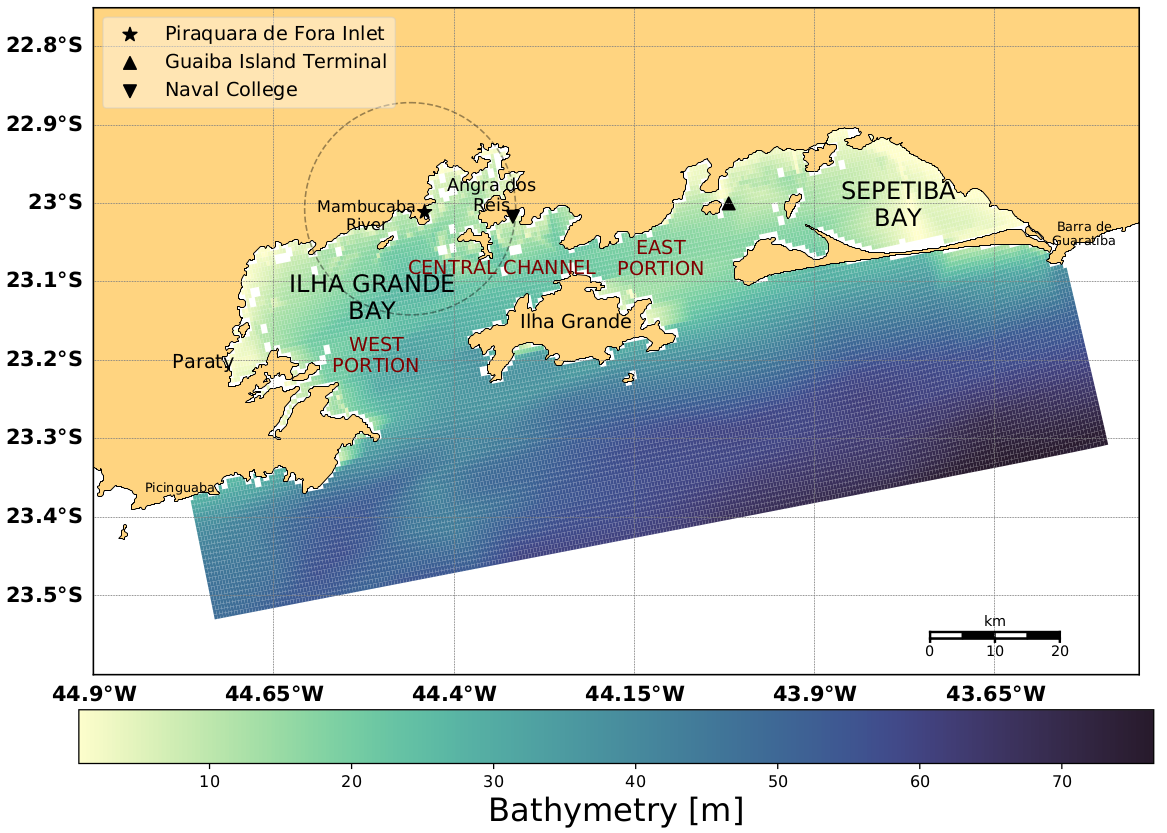
\includegraphics[width=0.8\columnwidth]{/home/tparente/danilo/mestrado/github/congressos/iwmo2018/figs/fig1.png}
\vspace{.1in}
\caption{The Ilha Grande and Sepetiba Bay domain used for ECOM model runs, showing bathymetry in meters. Several sites that are discussed in the paper are shown.}
\label{fig:areaestudo}
\end{figure}
% \vskip1ex
\vspace{-.5in}
% ===================================================================================================================
\section{Methods}

\vskip1ex
\begin{figure}
\centering
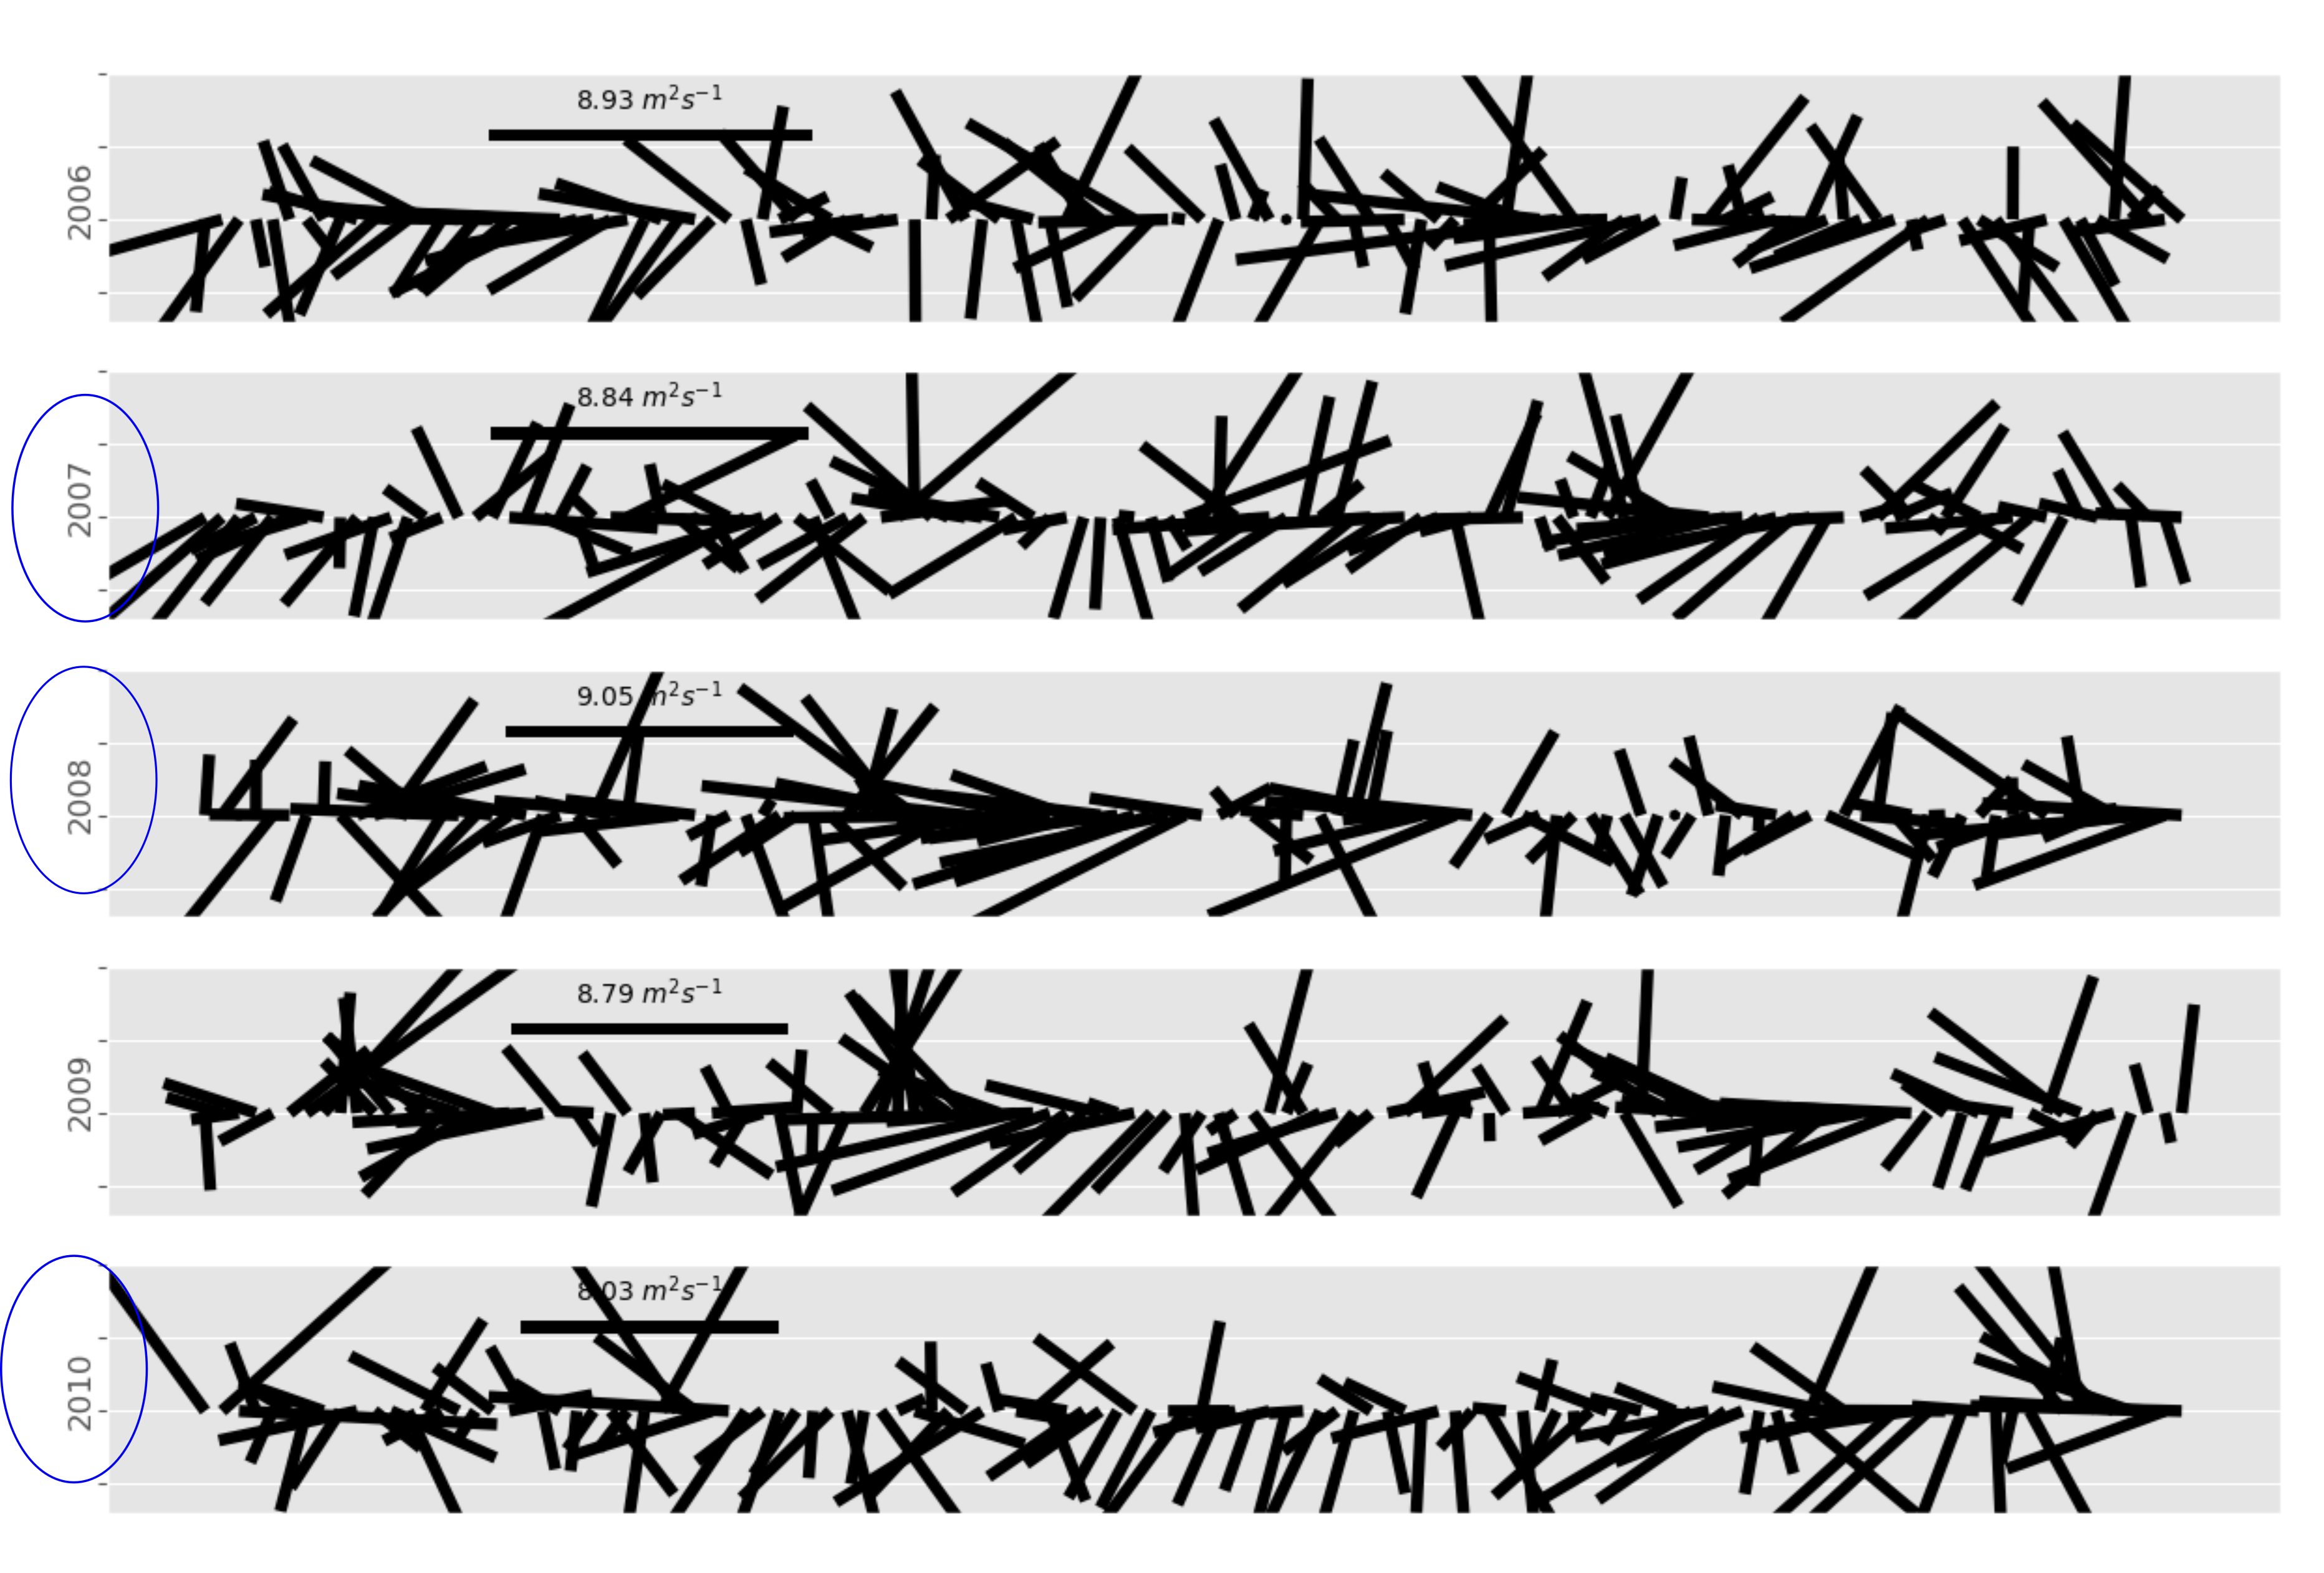
\includegraphics[width=0.9\columnwidth]{/home/tparente/danilo/mestrado/github/congressos/iwmo2018/figs/fig2.png}
\vspace{.2in}
\caption{Method applied in this work, where red boxes represent all input data, black boxes indicate the modules from ECOM, blue boxes represent the experiments used to analyze the influece of each forcing and green boxes represent the experiments used to analyze the dispersion.}
\label{fig:metodologia}
\end{figure}
\vskip1ex



\vspace{-.7in}
% ===================================================================================================================

\section{Results and Discussions}

\subsection{Wind v. Tide: Surface Circulation}

It was observed an intense eastward current in central channel in Experiment I, with northeasterly winds, 
associated to the South America Subtropical High, reaching velocities close to 0.25 m.s$^{-1}$, while in Experiment II, 
with winds associated to Frontal Systems passage, such currents reach a maximum of 0.23 m.s$^{-1}$, with a westward direction. 
The difference between these two experiments, considering the same wind intensity, may be caused by the open area available 
for southwesterly wind to act. Finally, Experimet III, only with tides from TPXO 7.2, presented the highest velocities, 
concentrated in the eastern region of the domain, with maximum velocities of 0.6 m.s$^{-1}$ during flood spring tide.

\vskip1ex
\begin{figure}
\centering
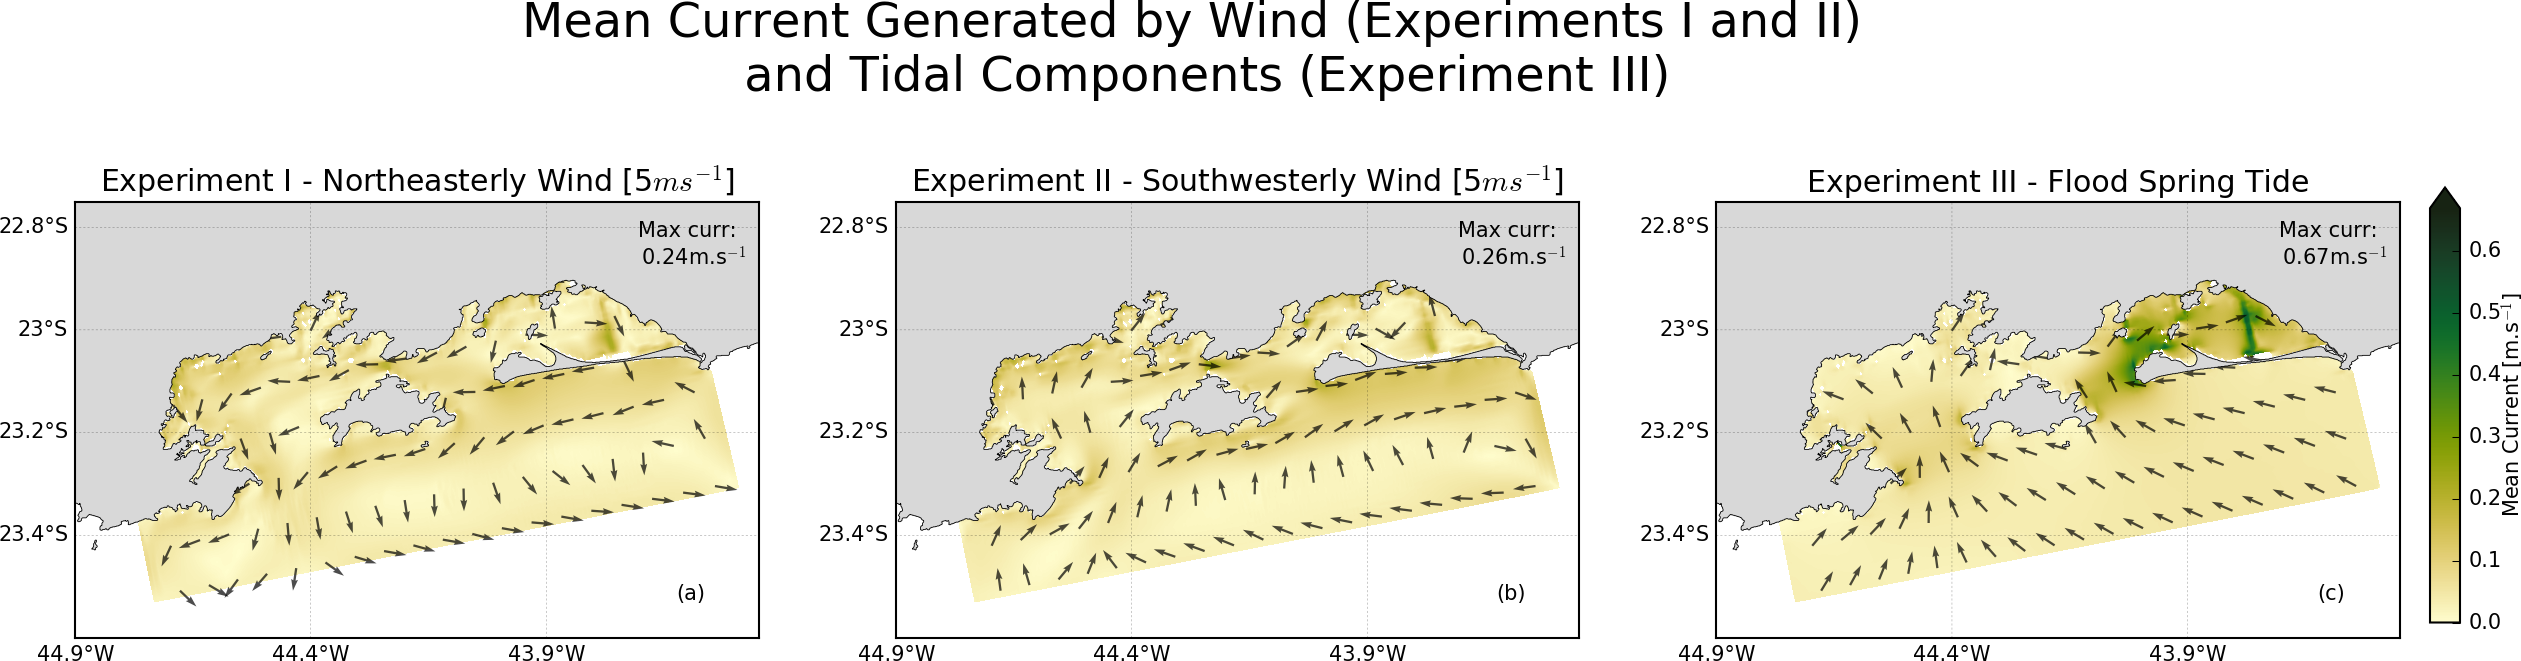
\includegraphics[width=1.\columnwidth]{/home/tparente/danilo/mestrado/github/congressos/iwmo2018/figs/fig3.png}
\caption{Mean current no Experiments I, II and III. Panels (a) and (b) represent the current in the last instant modelled and panel (c) represent the flooding spring tides.}
\label{fig:cenariosCirc}
\end{figure}
\vspace{-1ex}

In Experiments V and VI all variables are used (tide, wind and fluvial discharge), with
variable winds based on typical values, like in Experiments I and II, respectively. 
In these scenarios, we identify that southwesterly winds induce the strongest surface
currents, with mean values of 0.43 m.s$^{-1}$ (Figure~\ref{fig:cenariosDispersao}.a 
and~\ref{fig:cenariosDispersao}.b). Despite the influence of the tides in more intense currents, 
the surface current direction will be controlled by the direction of the wind 
(Figure~\ref{fig:cenariosDispersao}.c and~\ref{fig:cenariosDispersao}.d), 
consequenty, controlling the direction of the radioactive material dispersion.
The tide, in this case, will be the main mechanism acting on mixing of radioactive the
material.

\vskip.2ex
\begin{figure}
\centering
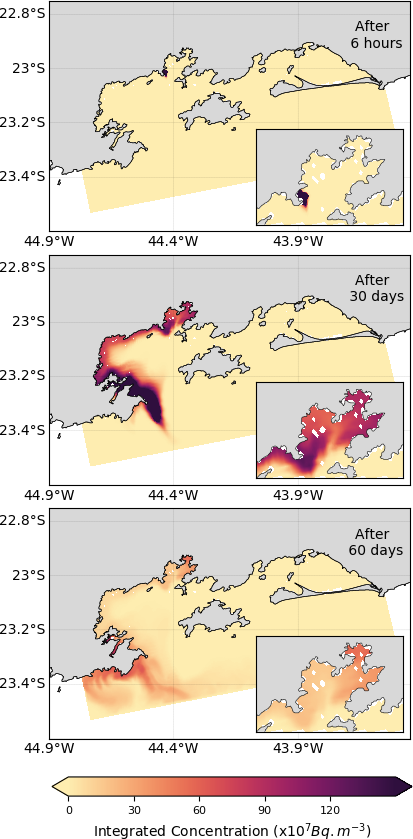
\includegraphics[width=0.99\columnwidth]{/home/tparente/danilo/mestrado/github/congressos/iwmo2018/figs/fig4.png}
\caption{Mean surface current on the upper panels and integrated dispersion on the inferior panels.}
\label{fig:cenariosDispersao}
\end{figure}

\subsection{Dispersion in a Scenario Under Closest to Real Conditions}


A simulation using real wind inputs shoewd that the radioactive material is transported 
to the east, reaching areas with more intense currents and, consequently, with a
greater mixing of the pollutant. Locally, the material will stay in the northwest 
of Angra dos Reis, region where the higher concentrations in the surface sediment 
are found, corroborating with the information obtained through the hydrodynamics modelling.

\vskip.2ex
\begin{figure}
\centering
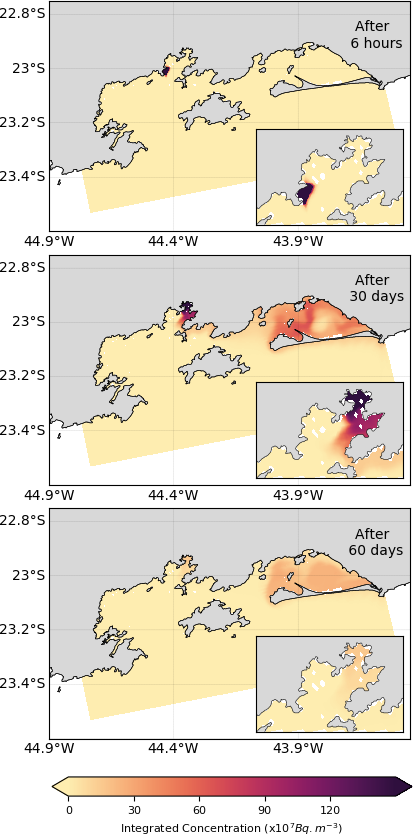
\includegraphics[width=0.9\columnwidth]{/home/tparente/danilo/mestrado/github/congressos/iwmo2018/figs/fig5.png}
\caption{Temporal evolution of the radioactive material under spatial and temporal wind variations.}
\label{fig:evolucaopluma}
\end{figure}
% \vskip2ex

% ===================================================================================================================
\vspace{-.5in}
\section{Conclusions}

\begin{itemize}
	\item Wind controls direction;
	\item Tide controls the mixing;
	\item In real wind and tide condition, the plume evolves to regions with more intense currents;
	\item The most impacted region is Angra dos Reis, followed by Central Channel and 
	Mambucada River and
	\item The East Portion is the main area of mixing.
\end{itemize}

\end{multicols}

%==============================================================================
\end{frame}
\end{document}
